\clearpage
\subsection{Device-Level Attribution}
\label{sec:eval:analysis}

\input{tables/benefits-all}

\begin{figure}[H]
	\centering
	\begin{subfigure}[t]{0.40\textwidth}
		\centering
		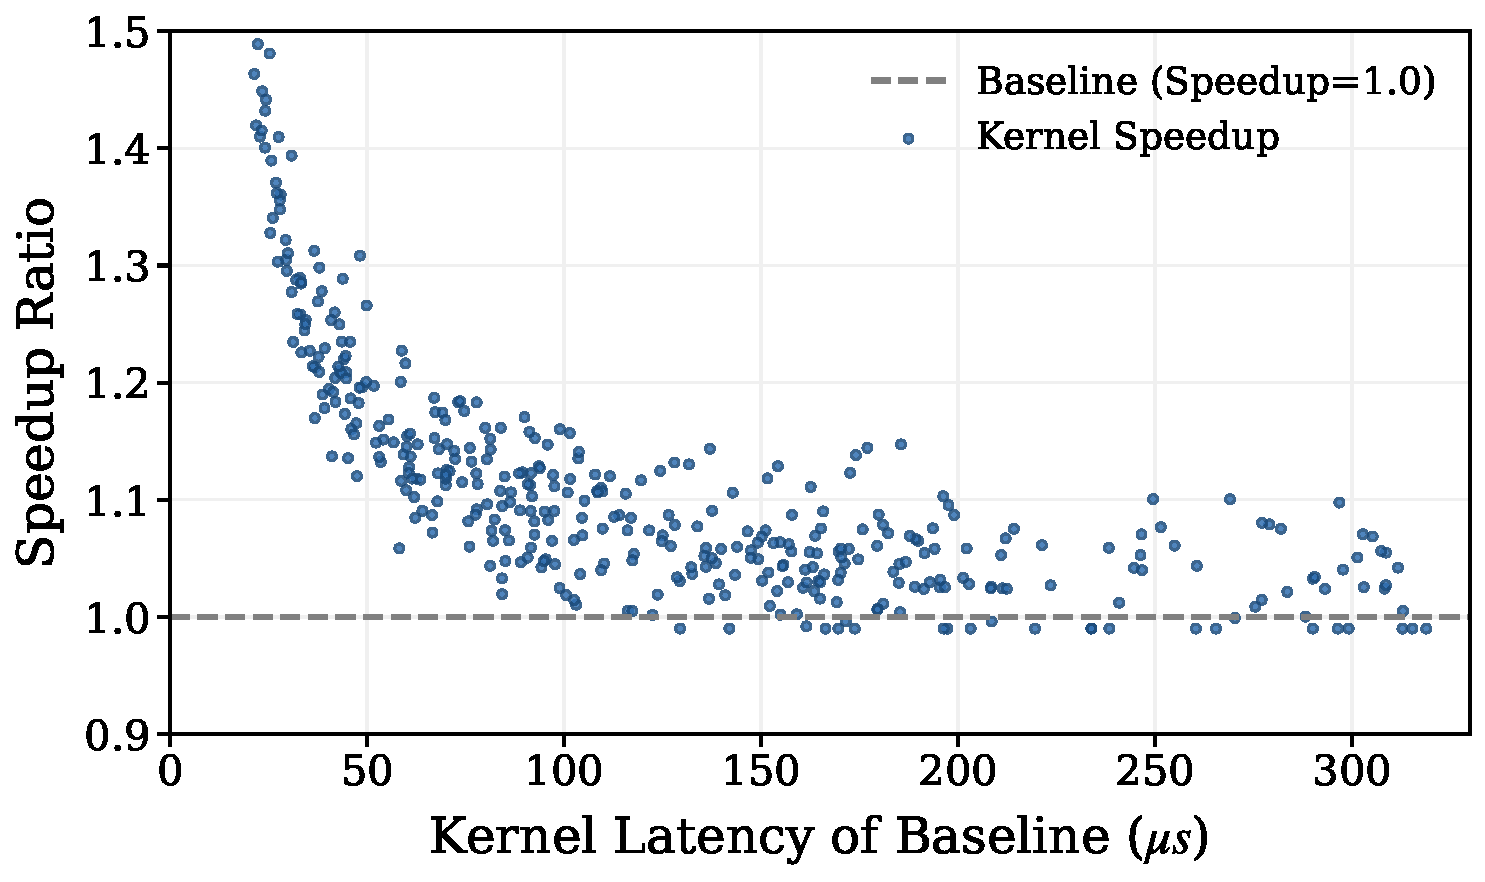
\includegraphics[width=\linewidth]{figures/evaluation/op-speedup/d_attn_execution_speedup.pdf}
		\caption{D-Attn}
	\end{subfigure}
	\hfill
	\begin{subfigure}[t]{0.40\textwidth}
		\centering
		\includegraphics[width=\linewidth]{figures/evaluation/op-speedup/mm_execution_speedup.pdf}
		\caption{MM}
	\end{subfigure}
	\caption{Kernel speedup versus Baseline device-kernel latency for D-Attn and MM. Blue points report the speedup of TilingInfer relative to Baseline.}
	\Description{Two scatter plots showing TilingInfer kernel speedup versus Baseline device-kernel latency for D-Attn and MM.}
	\label{fig:eval:op-scaling}
\end{figure}

\FloatBarrier

{\color{red}%
\DIFdel{%
To gain deeper insight into the sources of performance gains demonstrated in Section~}\ref{sec:eval:result}\DIFdel{, we analyze low-level hardware performance metrics collected during operator execution. }\autoref{tab:performance_metrics}\DIFdel{ details the Speedup alongside key architectural metrics: Instruction Cache (I-Cache) Miss Rate, Scalar Instruction Ratio, Memory Access (Read and Write) Ratios, and the final compiled Binary Size. The Scalar Ratio, Memory Read Ratio, and Memory Write Ratio quantify the proportion of execution cycles of corresponding hardware units (scalar units, memory read/write units) relative to the total kernel execution cycles. Comparing TilingInfer (T) against the Baseline (B) and LLVM-spec (L), we attribute the improvements to two primary factors: reduced instruction fetch overhead and simplified runtime calculation.
}
\par}

{\color{red}%
\DIFdel{%
Reduction in Binary Size and I-Cache Misses. By propagating runtime invariants, TilingInfer enables the backend compiler to aggressively perform Dead Code Elimination (DCE) and simplify control flow graphs. This leads to significant binary size reductions: 34.0\% for Upsample, 22.7\% for D-Attn, 20.2\% for FFN, and 14.8\% for P-Attn. Consequently, the I-Cache Miss rate drops substantially: Upsample (9.83\% $\rightarrow$ 0.12\%), D-Attn (4.45\% $\rightarrow$ 0.18\%), FFN (3.89\% $\rightarrow$ 0.15\%), and P-Attn (16.40\% $\rightarrow$ 11.39\%). These improvements in instruction fetch efficiency contribute to the observed speedups.
}
\par}

{\color{red}%
\DIFdel{%
Optimization of Computational Intensity and Memory Schedule. TilingInfer substantially reduces the Scalar Ratio for operators like RMS (97.9\% $\rightarrow$ 88.6\%) and Pow (59.5\% $\rightarrow$ 53.1\%), confirming that resolving loop bounds and offsets at compile time effectively converts runtime scalar calculations into immediate operands. The Memory Read Ratio also improves, dropping from 25.0\% to 16.4\% for Gate and from 25.0\% to 18.8\% for GN. This reduction is primarily due to the decreased number of parameters read from device memory, as well as the compiler's ability to merge multiple memory accesses when loop iteration counts are determined at compile time. Furthermore, optimizations such as loop unrolling can facilitate instruction scheduling and effectively hide memory access latency. These factors collectively contribute to the speedups observed in operators such as D-Attn, Pow, and RMS.
}
\par}

{\color{red}%
\DIFdel{%
Insensitive Operators. Some operators, such as Pool and Scat, show negligible speedups (1.00$\times$--1.01$\times$). For Pool, the Baseline binary size is already minimal (13.35KB) with 0.08\% I-Cache miss rate, leaving no room for control flow simplification. For Scat, the overhead of scalar instructions and instruction fetching is minimal compared to memory-bound operations. Optimizations in the instruction stream do not translate into visible latency reductions when the bottleneck lies in memory or arithmetic units.
}
\par}

{\color{red}%
\DIFdel{%
Impact of Workload Scale. The original varying-KV-length and latency-distribution results show that speedup decreases towards 1.0 as workload increases. This implies that performance benefits from kernel specialization are relatively fixed in absolute time. Consequently, this fixed reduction yields significant speedup ratios for small-scale kernels but becomes negligible for heavy workloads dominated by computation and memory access.
}
\par}

{\color{blue}%
\autoref{tab:performance_metrics} and \autoref{fig:eval:op-scaling} show that TilingInfer does not produce uniform device-level gains; benefiting kernels fall into two mechanism-driven classes, whereas a third class is largely insensitive. For Upsample, D-Attn, FFN, and P-Attn, gains mainly arise because invariant propagation exposes constant branches and loop structure, enabling dead-code elimination and control-flow simplification; the resulting smaller instruction footprint reduces instruction-fetch and I-Cache pressure. A second class, including RMS, Pow, Gate, and GN, benefits primarily from simplified runtime calculation and memory scheduling. Resolving loop bounds, offsets, and schedule parameters removes scalar loads and address or control computations, exposes immediate operands, and enables access merging, loop unrolling, and more effective instruction scheduling. In contrast, Pool and Scat are largely insensitive: Pool is already compact with little instruction-fetch overhead, whereas Scat is dominated by memory work, so instruction-stream simplification does not shorten the critical path. Across all three classes, specialization mainly removes a roughly fixed amount of control and scheduling overhead. Its relative effect is therefore strongest for short-running kernels and diminishes as tensor computation or memory traffic dominates. The key determinant is not whether a parameter is static, but whether resolving it eliminates work on the kernel's performance-critical path.
\par}
